% documentclass: article used for scientific journals, short reports, program documentation, etc
% options: fontsize 11, generate document for double sided printing, a4-paper
\documentclass[11pt, twoside, a4paper]{article}

% package for changing page layout
\usepackage{geometry}
\geometry{a4paper, lmargin=30mm, rmargin=20mm, tmargin=30mm, bmargin=20mm}
% set indentation
\setlength{\parindent}{0mm} 

% input encoding for special characters (e.g. ä,ü,ö,ß), only for non english text
% options: utf8 as encoding standard
\usepackage[utf8]{inputenc}
% package for changing used language
% options: german or default: english
\usepackage[german]{babel}

% package for math symbols, functions and environments from ams(american mathematical society)
\usepackage{amsmath}
% package for extended symbols from ams
\usepackage{amssymb}
% package for extended symbols from stmaryrd(st mary road)
%\usepackage{stmaryrd}
% package for managing pictures
\usepackage{graphicx}

% package for some extra fonts
\usepackage{txfonts}
% package for changing color of font and paper
% options: using names of default colors (e.g red, black)
\usepackage[usenames]{color}

% package for converting eps-files to pdf-files and then include them
\usepackage{epstopdf}
% use another program (ps2pdf) for converting
% !!! important: set shell_escape=1 in /etc/texmf/texmf.cnf (Linux) for allowing to use other programs
% !!!			 or use the command line with -shell-escape
\epstopdfDeclareGraphicsRule{.eps}{pdf}{.pdf}{
ps2pdf -dEPSCrop #1 \OutputFile
}

% package for reference to last page (output number of last page)
\usepackage{lastpage}
% package for using header and footer
% options: automate terms of right and left marks
\usepackage[automark]{scrpage2}
% set style for footer and header
\pagestyle{scrheadings}
% clear pagestyle for redefining
\clearscrheadfoot
% set header and footer: use <xx>head/foot[]{Text} (i...inner, o...outer, c...center, o...odd, e...even, l...left, r...right)
\ihead[]{}
\ohead[]{}
\cfoot[]{\pagemark/\pageref{LastPage}}


% begin the document
\begin{document}
	
	\begin{figure}[h]
		\center
		% GNUPLOT: LaTeX picture with Postscript
\begingroup
  \makeatletter
  \providecommand\color[2][]{%
    \GenericError{(gnuplot) \space\space\space\@spaces}{%
      Package color not loaded in conjunction with
      terminal option `colourtext'%
    }{See the gnuplot documentation for explanation.%
    }{Either use 'blacktext' in gnuplot or load the package
      color.sty in LaTeX.}%
    \renewcommand\color[2][]{}%
  }%
  \providecommand\includegraphics[2][]{%
    \GenericError{(gnuplot) \space\space\space\@spaces}{%
      Package graphicx or graphics not loaded%
    }{See the gnuplot documentation for explanation.%
    }{The gnuplot epslatex terminal needs graphicx.sty or graphics.sty.}%
    \renewcommand\includegraphics[2][]{}%
  }%
  \providecommand\rotatebox[2]{#2}%
  \@ifundefined{ifGPcolor}{%
    \newif\ifGPcolor
    \GPcolorfalse
  }{}%
  \@ifundefined{ifGPblacktext}{%
    \newif\ifGPblacktext
    \GPblacktexttrue
  }{}%
  % define a \g@addto@macro without @ in the name:
  \let\gplgaddtomacro\g@addto@macro
  % define empty templates for all commands taking text:
  \gdef\gplbacktext{}%
  \gdef\gplfronttext{}%
  \makeatother
  \ifGPblacktext
    % no textcolor at all
    \def\colorrgb#1{}%
    \def\colorgray#1{}%
  \else
    % gray or color?
    \ifGPcolor
      \def\colorrgb#1{\color[rgb]{#1}}%
      \def\colorgray#1{\color[gray]{#1}}%
      \expandafter\def\csname LTw\endcsname{\color{white}}%
      \expandafter\def\csname LTb\endcsname{\color{black}}%
      \expandafter\def\csname LTa\endcsname{\color{black}}%
      \expandafter\def\csname LT0\endcsname{\color[rgb]{1,0,0}}%
      \expandafter\def\csname LT1\endcsname{\color[rgb]{0,1,0}}%
      \expandafter\def\csname LT2\endcsname{\color[rgb]{0,0,1}}%
      \expandafter\def\csname LT3\endcsname{\color[rgb]{1,0,1}}%
      \expandafter\def\csname LT4\endcsname{\color[rgb]{0,1,1}}%
      \expandafter\def\csname LT5\endcsname{\color[rgb]{1,1,0}}%
      \expandafter\def\csname LT6\endcsname{\color[rgb]{0,0,0}}%
      \expandafter\def\csname LT7\endcsname{\color[rgb]{1,0.3,0}}%
      \expandafter\def\csname LT8\endcsname{\color[rgb]{0.5,0.5,0.5}}%
    \else
      % gray
      \def\colorrgb#1{\color{black}}%
      \def\colorgray#1{\color[gray]{#1}}%
      \expandafter\def\csname LTw\endcsname{\color{white}}%
      \expandafter\def\csname LTb\endcsname{\color{black}}%
      \expandafter\def\csname LTa\endcsname{\color{black}}%
      \expandafter\def\csname LT0\endcsname{\color{black}}%
      \expandafter\def\csname LT1\endcsname{\color{black}}%
      \expandafter\def\csname LT2\endcsname{\color{black}}%
      \expandafter\def\csname LT3\endcsname{\color{black}}%
      \expandafter\def\csname LT4\endcsname{\color{black}}%
      \expandafter\def\csname LT5\endcsname{\color{black}}%
      \expandafter\def\csname LT6\endcsname{\color{black}}%
      \expandafter\def\csname LT7\endcsname{\color{black}}%
      \expandafter\def\csname LT8\endcsname{\color{black}}%
    \fi
  \fi
  \setlength{\unitlength}{0.0500bp}%
  \begin{picture}(8502.00,5102.00)%
    \gplgaddtomacro\gplbacktext{%
      \csname LTb\endcsname%
      \put(814,704){\makebox(0,0)[r]{\strut{}0.0}}%
      \put(814,1327){\makebox(0,0)[r]{\strut{}0.2}}%
      \put(814,1950){\makebox(0,0)[r]{\strut{}0.4}}%
      \put(814,2573){\makebox(0,0)[r]{\strut{}0.6}}%
      \put(814,3195){\makebox(0,0)[r]{\strut{}0.8}}%
      \put(814,3818){\makebox(0,0)[r]{\strut{}1.0}}%
      \put(814,4441){\makebox(0,0)[r]{\strut{}1.2}}%
      \put(946,484){\makebox(0,0){\strut{} 400}}%
      \put(1662,484){\makebox(0,0){\strut{} 425}}%
      \put(2378,484){\makebox(0,0){\strut{} 450}}%
      \put(3094,484){\makebox(0,0){\strut{} 475}}%
      \put(3810,484){\makebox(0,0){\strut{} 500}}%
      \put(4526,484){\makebox(0,0){\strut{} 525}}%
      \put(5241,484){\makebox(0,0){\strut{} 550}}%
      \put(5957,484){\makebox(0,0){\strut{} 575}}%
      \put(6673,484){\makebox(0,0){\strut{} 600}}%
      \put(7389,484){\makebox(0,0){\strut{} 625}}%
      \put(8105,484){\makebox(0,0){\strut{} 650}}%
      \put(176,2572){\rotatebox{-270}{\makebox(0,0){\strut{}qualitative Intensität}}}%
      \put(4525,154){\makebox(0,0){\strut{}$\lambda \ [nm]$}}%
      \put(4525,4771){\makebox(0,0){\strut{}Hg-Spektrum}}%
      \put(1290,2261){\makebox(0,0)[l]{\strut{}violett}}%
      \put(2091,2884){\makebox(0,0)[l]{\strut{}blau}}%
      \put(3523,2261){\makebox(0,0)[l]{\strut{}blaugrün}}%
      \put(5241,4130){\makebox(0,0)[l]{\strut{}grün}}%
      \put(6387,3507){\makebox(0,0)[l]{\strut{}gelb}}%
      \put(7532,1638){\makebox(0,0)[l]{\strut{}rot}}%
    }%
    \gplgaddtomacro\gplfronttext{%
    }%
    \gplbacktext
    \put(0,0){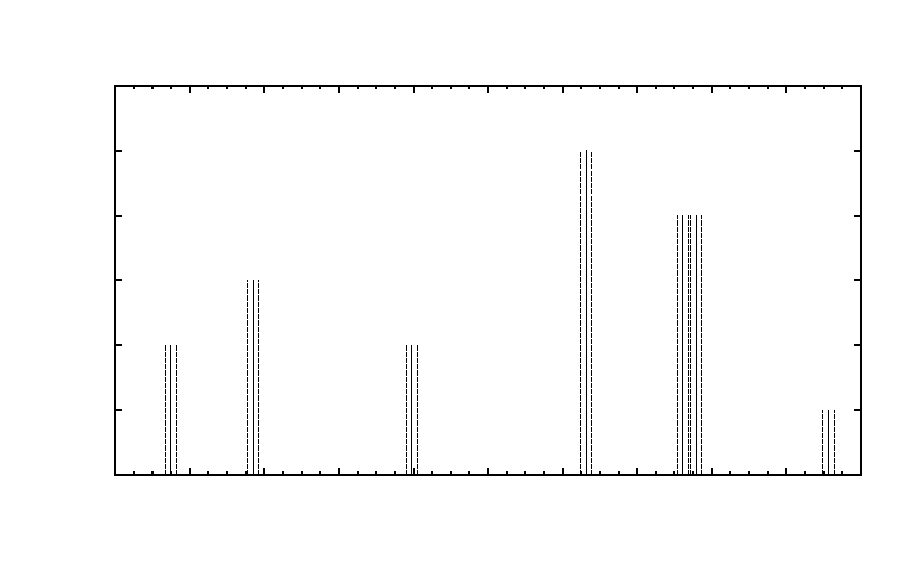
\includegraphics{hg-spektrum}}%
    \gplfronttext
  \end{picture}%
\endgroup

	\end{figure}

	\begin{figure}[h]
		\center
		% GNUPLOT: LaTeX picture with Postscript
\begingroup
  \makeatletter
  \providecommand\color[2][]{%
    \GenericError{(gnuplot) \space\space\space\@spaces}{%
      Package color not loaded in conjunction with
      terminal option `colourtext'%
    }{See the gnuplot documentation for explanation.%
    }{Either use 'blacktext' in gnuplot or load the package
      color.sty in LaTeX.}%
    \renewcommand\color[2][]{}%
  }%
  \providecommand\includegraphics[2][]{%
    \GenericError{(gnuplot) \space\space\space\@spaces}{%
      Package graphicx or graphics not loaded%
    }{See the gnuplot documentation for explanation.%
    }{The gnuplot epslatex terminal needs graphicx.sty or graphics.sty.}%
    \renewcommand\includegraphics[2][]{}%
  }%
  \providecommand\rotatebox[2]{#2}%
  \@ifundefined{ifGPcolor}{%
    \newif\ifGPcolor
    \GPcolorfalse
  }{}%
  \@ifundefined{ifGPblacktext}{%
    \newif\ifGPblacktext
    \GPblacktexttrue
  }{}%
  % define a \g@addto@macro without @ in the name:
  \let\gplgaddtomacro\g@addto@macro
  % define empty templates for all commands taking text:
  \gdef\gplbacktext{}%
  \gdef\gplfronttext{}%
  \makeatother
  \ifGPblacktext
    % no textcolor at all
    \def\colorrgb#1{}%
    \def\colorgray#1{}%
  \else
    % gray or color?
    \ifGPcolor
      \def\colorrgb#1{\color[rgb]{#1}}%
      \def\colorgray#1{\color[gray]{#1}}%
      \expandafter\def\csname LTw\endcsname{\color{white}}%
      \expandafter\def\csname LTb\endcsname{\color{black}}%
      \expandafter\def\csname LTa\endcsname{\color{black}}%
      \expandafter\def\csname LT0\endcsname{\color[rgb]{1,0,0}}%
      \expandafter\def\csname LT1\endcsname{\color[rgb]{0,1,0}}%
      \expandafter\def\csname LT2\endcsname{\color[rgb]{0,0,1}}%
      \expandafter\def\csname LT3\endcsname{\color[rgb]{1,0,1}}%
      \expandafter\def\csname LT4\endcsname{\color[rgb]{0,1,1}}%
      \expandafter\def\csname LT5\endcsname{\color[rgb]{1,1,0}}%
      \expandafter\def\csname LT6\endcsname{\color[rgb]{0,0,0}}%
      \expandafter\def\csname LT7\endcsname{\color[rgb]{1,0.3,0}}%
      \expandafter\def\csname LT8\endcsname{\color[rgb]{0.5,0.5,0.5}}%
    \else
      % gray
      \def\colorrgb#1{\color{black}}%
      \def\colorgray#1{\color[gray]{#1}}%
      \expandafter\def\csname LTw\endcsname{\color{white}}%
      \expandafter\def\csname LTb\endcsname{\color{black}}%
      \expandafter\def\csname LTa\endcsname{\color{black}}%
      \expandafter\def\csname LT0\endcsname{\color{black}}%
      \expandafter\def\csname LT1\endcsname{\color{black}}%
      \expandafter\def\csname LT2\endcsname{\color{black}}%
      \expandafter\def\csname LT3\endcsname{\color{black}}%
      \expandafter\def\csname LT4\endcsname{\color{black}}%
      \expandafter\def\csname LT5\endcsname{\color{black}}%
      \expandafter\def\csname LT6\endcsname{\color{black}}%
      \expandafter\def\csname LT7\endcsname{\color{black}}%
      \expandafter\def\csname LT8\endcsname{\color{black}}%
    \fi
  \fi
  \setlength{\unitlength}{0.0500bp}%
  \begin{picture}(8502.00,5102.00)%
    \gplgaddtomacro\gplbacktext{%
      \csname LTb\endcsname%
      \put(1078,704){\makebox(0,0)[r]{\strut{}1.615}}%
      \put(1078,1119){\makebox(0,0)[r]{\strut{}1.620}}%
      \put(1078,1534){\makebox(0,0)[r]{\strut{}1.625}}%
      \put(1078,1950){\makebox(0,0)[r]{\strut{}1.630}}%
      \put(1078,2365){\makebox(0,0)[r]{\strut{}1.635}}%
      \put(1078,2780){\makebox(0,0)[r]{\strut{}1.640}}%
      \put(1078,3195){\makebox(0,0)[r]{\strut{}1.645}}%
      \put(1078,3611){\makebox(0,0)[r]{\strut{}1.650}}%
      \put(1078,4026){\makebox(0,0)[r]{\strut{}1.655}}%
      \put(1078,4441){\makebox(0,0)[r]{\strut{}1.660}}%
      \put(1210,484){\makebox(0,0){\strut{}400}}%
      \put(2589,484){\makebox(0,0){\strut{}450}}%
      \put(3968,484){\makebox(0,0){\strut{}500}}%
      \put(5347,484){\makebox(0,0){\strut{}550}}%
      \put(6726,484){\makebox(0,0){\strut{}600}}%
      \put(8105,484){\makebox(0,0){\strut{}650}}%
      \put(176,2572){\rotatebox{-270}{\makebox(0,0){\strut{}$n \ [1]$}}}%
      \put(4657,154){\makebox(0,0){\strut{}$\lambda \ [nm]$}}%
      \put(4657,4771){\makebox(0,0){\strut{}Dispersionskurve $n(\lambda)$}}%
      \put(5347,3611){\makebox(0,0)[l]{\strut{}$a = (6.5 \pm 1.0) \ 10^{-7} \ nm^{-2}$}}%
      \put(5347,3195){\makebox(0,0)[l]{\strut{}$b = (-8.5 \pm 1.1) \ 10^{-4} \ nm^{-1}$}}%
      \put(5347,2780){\makebox(0,0)[l]{\strut{}$c = (1.893 \pm 0.028)$}}%
    }%
    \gplgaddtomacro\gplfronttext{%
      \csname LTb\endcsname%
      \put(7118,4246){\makebox(0,0)[r]{\strut{}Messwerte}}%
      \csname LTb\endcsname%
      \put(7118,3982){\makebox(0,0)[r]{\strut{}$f(x)=ax^2+bx+c$}}%
    }%
    \gplbacktext
    \put(0,0){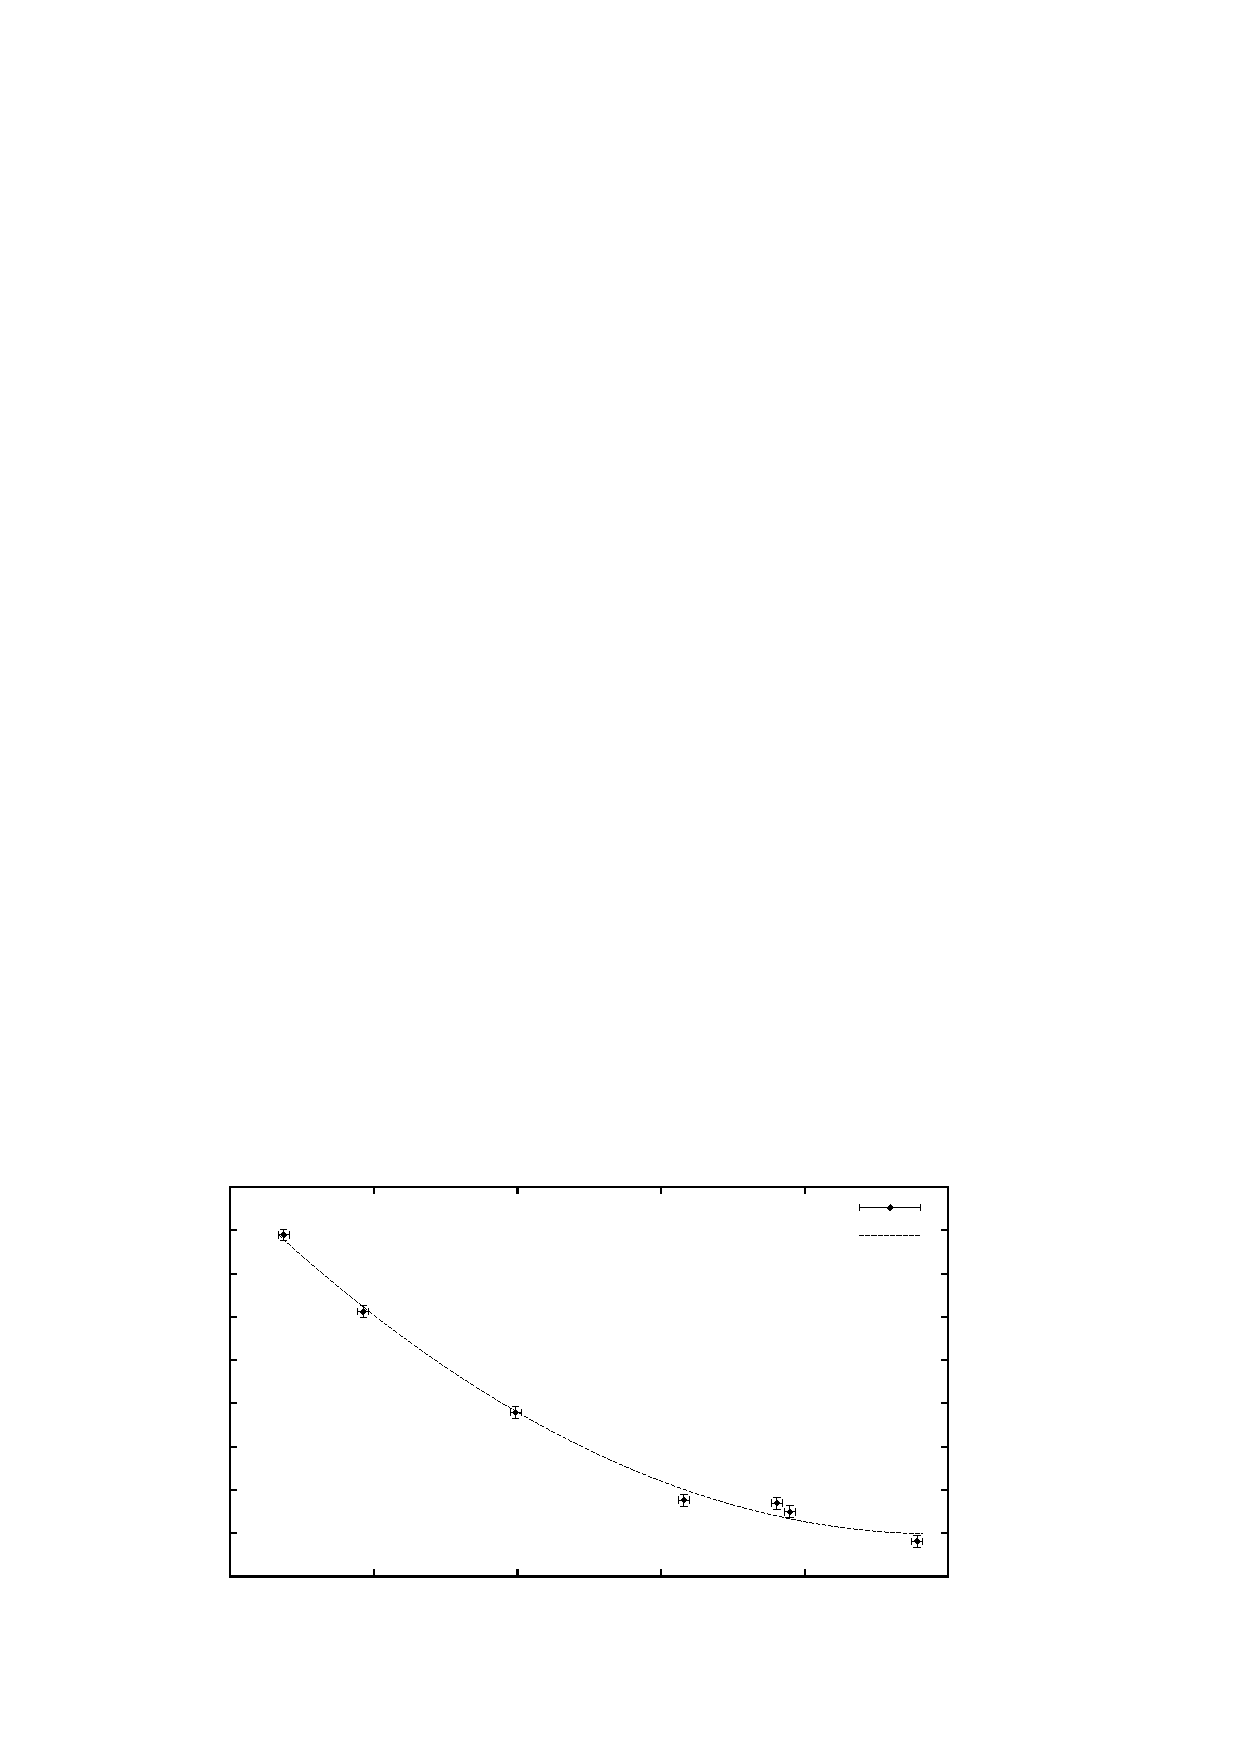
\includegraphics{dispersion}}%
    \gplfronttext
  \end{picture}%
\endgroup

	\end{figure}
	
\end{document}

